
%FILL IN THE RIGHT INFO.
%\lecture{**LECTURE-NUMBER**}{**DATE**}
\unchapter{Lecture 19}
\lecture{19}{November 5}
\setcounter{section}{0}
\setcounter{theorem}{0}

% **** YOUR NOTES GO HERE:


We dedicate this lecture to the proof of existence in theorem (\ref{thm:r-map-thm}).

\section{Proof of RMT}


\begin{proof}[Existence in \ref{thm:r-map-thm}]
Let $\oic$ non-empty, $\om \neq \C$, satisfying that $\forall \, \foc, \; \exists \, F: \om \to \C$ antiderivative for $f$ (in particular, this is satisfied if $\om $ is simply connected). We want to find a biholomorphism $f:\om \to D$ such that for some fixed $z_0 \in \om$, $f(z_0) = 0$. We reduce this proof into 3 steps.
\begin{enumerate}

\subsection{Step 1}

    \item In this step we will reduce $\om$ to a subset of $D$ by showing that there is a biholomorphism between $\om$ and a subset of $D$. Furthermore, this biholomorphism can be constructed in such a way that $\om \ni z_0 \mapsto 0$. 
    
    To do this, note that $\om \neq \C$. Thus $\exists \, \alpha \in \C \setminus \om$. Then $z- \alpha$ is a holomorphic function on $\om$ that is never $0$, so since we assume that $\om$ satisfies the previously stated antiderivative property, it follows from theorem (\ref{thm:complex-log}) and theorem (\ref{thm:complex-log-super}) that $\exists \, g: \om \to \C$ holomorphic function such that:
    \begin{align*}
        e^{g(z)} = z - \alpha, \: \forall z \in \om.
    \end{align*}
    That is to say that $g$ is a branch of $\log(z-\alpha)$ ($g(z)$ is an antiderivative of $\frac{1}{z-\alpha}$).
    
    Some properties of $g$ include:
    \begin{itemize}
        \item $g$ is injective. To see this let $g(z_1) = g(z_2)$. Then $z_1 - \alpha = e^{g(z_1)} = e^{g(z_2)} = z_2 - \alpha$, so $z_1 = z_2$.
        \item given $w \in \om$, $g(z) \neq g(w) + 2 \pi i, \; \forall z \in \om$. To see this assume not. Then $\exists \, z \in \om$ s.t. $g(z) = g(w) + 2 \pi i$. Then $z - \alpha = e^{g(z)} = e^{g(w) + 2 \pi i}  = e^{g(w) } = w - \alpha$. Thus $z = w$, so $g(z) = g(w) \neq g(w) + 2 \pi i$ $\lightning$.
        
        
    \end{itemize}
    This means that given any $w \in \om$, $g(w) + 2 \pi i \not\in g(\om)$.
        
\begin{center}
    \begin{tikzpicture}[]
    
    \draw[scale =0.25]
        plot [smooth cycle] coordinates {(-10,0) (-7,3.5) (0,5)  (4,2.5) (7,0)  (5,-7) (2,-6)  (-5,-5) };


\draw[fill] (50:2) circle (0.08);
\draw[fill] (50:0) circle (0.08);

% \draw[shift=(175:2.75)][thick] (-0.1,0.1) -- (0.1,-0.1) (0.1,0.1) -- (-0.1,-0.1);


% \draw[shift=(-80:2)][thick] (-0.1,0.1) -- (0.1,-0.1) (0.1,0.1) -- (-0.1,-0.1);


% \draw[thick] (-0.1,0.1) -- (0.1,-0.1) (0.1,0.1) -- (-0.1,-0.1);
\draw (-45:0.0)[below right] node {$g(\omega)$};
\draw ($(50:2.0) + (-45:0.4)$)[below right] node {$g(\omega) + 2 \pi i$};
\draw (50:2) circle (0.5);
\draw (50:2) -- (50:2.5);
\draw ($(50:2.0) + (50:0.25)$)[below right] node {$\varepsilon$};

\draw node at (-2.25,-1) {$g(\Omega)$};


\end{tikzpicture}
\end{center}
        
    In fact, $\exists \, D_\varepsilon(g(w) + 2 \pi i)$ with $ g ( \om ) \cap  D_\varepsilon(g(w) + 2 \pi i) = \emptyset$. Indeed, if this doesn't hold, then $g(w) + 2 \pi i$ is not in the image, but is not separated by any disc from the image, and is therefore in the boundary of the image. Thus $\exists \{ z_n\} _{n=1} ^ \infty, \, z_n \in \om$ s.t. $g(z_n) \to g(w) + 2 \pi i$. But $z_n - \alpha = e^{g(z_n)} \to e^{g(w) + 2 \pi i} = e^{g(w)} = w - \alpha $. This implies that $z_n \to w$, thus $g(z_n) \to g(w)$. However by construction $g(z_n) \to g(w) + 2 \pi i \neq g(w)$.


\begin{remark}
Since $g:\om \to g(\om)$ is holomorphic and bijective, and since $g(\om)$ is open by the Open Mapping Theorem, $\om $ is biholomorphic to $g(\om)$ which ``misses a whole disk".

This is notable, in that there are simply connected sets that do not ``miss a whole disk", such as the slit plane. Applying this procedure to the slit plane, we get that the slit plane is biholomorphic to some set that misses a disk.
\end{remark}

Now that we know that we have missed a disk, we will naively apply ``$\frac{1}{z}$" to ``flip the inside and the outside of the disk. More precisely, pick any $w \in \om$. Let:

\begin{align*}
    F(z) \defas \frac{1}{g(z) - ( g( w) + 2 \pi i) }.
\end{align*}

Then $F$ has the following properties:
\begin{itemize}
    \item $F$ is holomorphic on $\om$, since $g(z) \neq g(w) + 2 \pi i, \; \forall z \in \om$.
    \item $F$ is injective on $\om$, since $F(z_1) = F(z_2) \Rightarrow g(z_1) = g(z_2) \Rightarrow z_1 = z_2$ (since $g$ is injective).
    \item Since $g(\om) \cap D_\varepsilon ( g(w) + 2 \pi i) = \varnothing$, then $\abs{g(z) - (g(w) + 2 \pi i)} \geq \varepsilon, \; \forall \, z \in \om$. That is to say that all points in the image of $g$ must lie at least $\varepsilon$ away from $g(w) + 2 \pi i$. Thus it follows that:
    \begin{align*}
        \abs{F(z)} = \frac{1}{\abs{g(z) - (g(w) + 2 \pi i)}} \leq \frac{1}{\varepsilon}, \; \forall \, z \in \om.
    \end{align*}
    
    Thus $F(\om) \subset \overline{D_\frac{1}{\varepsilon} (0)}$.
\end{itemize}

Thus $F: \om \to F(\om) \subset \overline{D_\frac{1}{\varepsilon} (0)} \subset D_\frac{2}{\varepsilon} (0)$ is holomorphic, bijective, and $F(\om)$ is open by the Open Mapping Theorem. Applying a biholomorphic rescaling $G: z \mapsto \frac{\varepsilon }{2} z$ we get:
\begin{align*}
    \om \xrightarrow[]{F} F(\om) \xrightarrow[]{G} G(F(\om)) \subset D_1(0).
\end{align*}

Since $F$ and $G$ are both biholomorphic, so is $F \circ G$. It follows that $\om$ is biholomorphic to $G(F(\om)) \subset D$ with $z_0 \mapsto G(F(z_0))$.

Finally we can scale and translate the image so that $z_0$ maps to $0$.

\begin{center}
    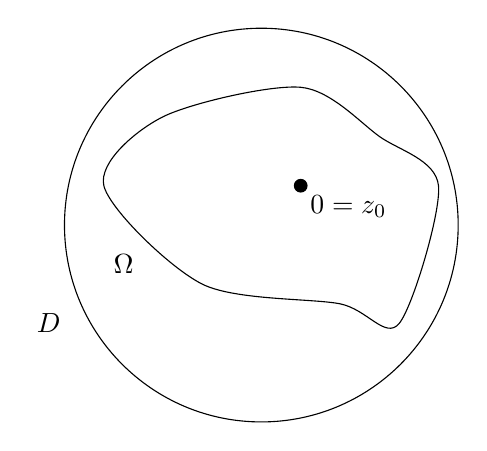
\begin{tikzpicture}[]
    
    \draw[scale =0.25]
        plot [smooth cycle] coordinates {(-10,0) (-7,3.5) (0,5)  (4,2.5) (7,0)  (5,-7) (2,-6)  (-5,-5) };


% \draw[fill] (50:2) circle (0.08);
\draw[fill] (50:0) circle (0.08);

% \draw[shift=(175:2.75)][thick] (-0.1,0.1) -- (0.1,-0.1) (0.1,0.1) -- (-0.1,-0.1);


% \draw[shift=(-80:2)][thick] (-0.1,0.1) -- (0.1,-0.1) (0.1,0.1) -- (-0.1,-0.1);


% \draw[thick] (-0.1,0.1) -- (0.1,-0.1) (0.1,0.1) -- (-0.1,-0.1);
\draw (-45:0.0)[below right] node {$0 = z_0$};

% \draw (50:2) circle (0.5);
% \draw (50:2) -- (50:2.5);
% \draw ($(50:2.0) + (50:0.25)$)[below right] node {$\varepsilon$};

\draw node at (-2.25,-1) {$\Omega$};
\draw (-0.5,-0.5) circle (2.5);
\draw node at (-3.2,-1.5)[below] {$D$};

\end{tikzpicture}
\end{center}

We are now done step one. We can relabel $F(G(\om))$ as $\om$, and similarly relabel $F(G(z_0))$ as $z_0$. 

\subsection{Step 2}

\item In this step we will find our biholomorphism $f: \om \to D$. The idea here is to look at a certain class of holomorphic functions and to maximize a certain property. $f$ will be found by solving a maximization problem over a well-chosen class of admissible holomorphic functions (this argument comes up frequently in the Calculus of Variations).

Let $\mathscr{F} = \set{ f: \om \to D \mid f \text{ holomorphic and injective, } f(0) = 0}$. Note that since $\om \subset D$, by step 1, $\mathscr{F}$ is not empty (as ($z\mapsto z$) $\in \mathscr{F}$). The $f$ we want to find will be in this class, since we want to find a holomorphic and bijective function $f$ such that $f(0) = 0$. It thus makes sense to look for our desired biholomorphism among the elements of $\mathscr{F}$. We shall find it by solving a maximization problem in $\mathscr{F}$ (at this point it is unclear what maximization problem to solve).

Observe that $\mathscr{F}$ is a normal family of holomorphic functions from $\om \to D$. Indeed $\forall \, f \in \mathscr{F}, \, \abs{f(z) } \leq 1, \, \forall \, z \in D$ by definition, and thus $\mathscr{F}$ is a uniformly bounded family. By theorem (\ref{thm:montel}), $\mathscr{F}$ is a normal family.

Observe that $\forall \, z \in \om$, choose some $\varepsilon > 0$ s.t. $D_\epsilon(z) \subset \om$. Then note that:
\begin{align*}
    L(\partial D_\varepsilon (z)) &= 2 \pi \varepsilon,\\
    \sup_{w \in \partial D_\varepsilon (z)} \frac{f(w)}{(w-z)^2} &\leq \frac{1}{\varepsilon^2}.
\end{align*}

Then by equation (\ref{eq:cauchy-int-fla}) we have that $\forall \, f \in \mathscr{F}$:
\begin{align*}
    f'(z) &= \frac{1}{2 \pi i} \int_{\partial D_\varepsilon (z)} \frac{f(w)}{(w-z)^2} \dif w,\\
\implies \abs{f'(z)} &\leq \frac{1}{2 \pi} \abs{\int_{\partial D_\varepsilon (z)} \frac{f(w)}{(w-z)^2} \dif w}\\
&\leq L(\partial D_\varepsilon (z)) \sup_{w \in \partial D_\varepsilon (z)} \frac{f(w)}{(w-z)^2} \leq \frac{1}{\varepsilon}.
\end{align*}


Applying this to $z=0$ we get that:
\begin{align*}
    \mathscr{S} \defas \sup_{f \in \mathscr{F}} \abs{f'(0)} < \infty.
\end{align*}

Thus we shall maximize the functional:
\begin{align*}
    \mathscr{D} : \, \mathscr{F} &\to \R_{\geq 0}\\
    f &\mapsto \abs{f'(0)},
\end{align*}
with
\begin{align*}
    \sup_{\mathscr{F}} & \mathscr{D} = \mathscr{S} < \infty.
\end{align*}

By the definition of $\sup$, $\exists \, \{ f_n\}_{n=1}^\infty, \; f_n \in \mathscr{F}$ s.t. $\abs{f_n' (0)} \xrightarrow[]{n \to \infty} \mathscr{S}$.

Recall that by theorem (\ref{thm:ascoli-arzela}), $\mathscr{F}$ normal implies that if you have a sequence in $\mathscr{F}$, you can pick a subsequence that converges uniformly on compact subsets to some limit function which is holomorphic, and in fact all the derivatives converge in the same fashion. Thus $\exists$ a subsequence $f_{n_j}$ s.t. $f_{n_j} \tou f $ and $f_{n_j}' \tou f' $ on compact subsets of $\om$ where $f: \om \to \overline{D}$ (the closure comes from the fact that taking a limit possibly destroys our strict inequality, so $\abs{f} \leq 1$) is holomorphic. Since $\abs{f_n' (0)} \xrightarrow[]{n \to \infty} \mathscr{S}$ and $\abs{f_n' (0)} \xrightarrow[]{n \to \infty} \abs{f'(0)}$, we have that $\abs{f'(0)} = \mathscr{S}$.

Note that since $\id  \in \mathscr{F}$ and $\abs{  \id '(0)  } = 1$ we have that $\mathscr{S} \geq 1$, so $\mathscr{S} \neq 0$. It follows that $f$ cannot be constant (otherwise $\abs{f'(0)} =0$). By example (\ref{ex:automorphism-mmp}), $f(\om) \subset D$ (ie $f$ maps to the disk, not the closure).

We claim that $f \in \mathscr{F}$:
\begin{itemize}
    \item $f: \om \to D$ is holomorphic is done.
    \item $f(0) = \lim_j f_{n_j} (0) = \lim_j 0 = 0$ is done.
    \item $f$ is injective is not done.
\end{itemize}

It thus remains to check that $f$ is injective.

\begin{lemma}\label{lem:r-mapping-thm-lem}
$\oic$ open, $\{f_n\}_{n=0}^\infty, \; f_n : \om \to \C$ holomorphic and injective. Suppose that $f_n \tou f$ on compact subsets of $\om$, where $\foc$ holomorphic. Then either $f$ is injective or $f$ is constant.
\end{lemma}

\begin{example}
$\om = \C$, $f_n(z) = \frac{z}{n}$. Then $f_n \tou 0$ which is constant.
\end{example}

\begin{proof}
For a contradiction suppose that $f$ is neither injective nor constant. In particular $\exists \, z_1 \neq z_2 \in \om$ s.t. $f(z_1) = f(z_2)$. Let $g_n \defas f_n(z) - f_n(z_1) \tou f(z) - f(z_1) = g(z)$. Then $g \nequiv 0$ since $f $ is non-constant. Note that $g(z_2) = 0$. Then $z_2$ is an isolated $0$ for $g$ of order $N \geq 1$. By theorem (\ref{thm:arg-princ}) (for some $\varepsilon>0$ small such that $g(w) \neq 0 \; \forall \, 0 < \abs{w - z_2} < \varepsilon$): %might be "logarithmic derivaive formula" instead
\begin{align*}
    1 \leq N = \frac{1}{2 \pi i } \int_{\partial D_\varepsilon (z_2)} \frac{g'(w)}{g(w)} \dif w.
\end{align*}

Since $g_n \to g$ locally uniformly, thus $g_n' \to g'$ locally uniformly. Thus:
\begin{align*}
    \frac{g_n'(w)}{g_n(w)} \to \frac{g'(w)}{g(w)} &\text{ uniformly for $w \in \partial D_\varepsilon (z_2)$}\\
    &\Downarrow.\\
    \frac{1}{2 \pi i } \int_{\partial D_\varepsilon (z_2)} \frac{g_n'(w)}{g_n(w)} \dif w &\to \frac{1}{2 \pi i } \int_{\partial D_\varepsilon (z_2)} \frac{g'(w)}{g(w)} \dif w \geq 1.
\end{align*}
The LHS is equal to the number of zeroes of $g_n$ inside $D_\varepsilon (z_2)$. But since $f_n$ is injective, $g_n$ has no zeroes in $D_\varepsilon (z_1)$, thus the $\text{LHS} = 0 \; \lightning$.
\end{proof}

It follows that our $f$ is injective, and hence $f \in \mathscr{F}$.

\subsection{Step 3}

\item In this step we show that $f$ must be surjective. In the last step we picked $f$ injective such that $\abs{f'(0)}$ is as large as possible (it is not clear yet how surjectivity follows from this).

Suppose for a contradiction that $f$ is not surjective, thus $\exists \, \alpha \in D$ s.t. $\alpha \notin f(\om)$. Consider $\psi_\alpha (z) = \frac{\alpha - z}{ 1 - \overline{\alpha} z}$. Consider then $\psi_\alpha \circ f : \om \to D$. Then $\psi_\alpha ( f(\om))$ satisfies our assumption about the existence of antiderivatives (since $\psi_\alpha ( f(\om))$  is biholomorphic to $\om$). Further note that $\alpha \notin f(\om) \iff 0 \notin \psi_\alpha ( f(\om))$. By the antiderivative assumption, $\exists$ a branch of $\log(z) $ on $\psi_\alpha ( f(\om))$. Then define $g ( z) \defas e^{\frac{1}{2} \log(z)}$ a branch of $\sqrt{z}$ on $\psi_\alpha ( f(\om))$.

The key trick is to now examine:
\begin{align*}
    F \defas \psi_{g(\alpha)} \circ g \circ \psi_\alpha \circ f.
\end{align*}
This is a holomorphic function from $\om \to D$ with $F(0) = 0$ (recalling that $f(0) = 0$). The goal will be to show that $F \in \mathscr{F}$, and that $\abs{F'(0)} > \abs{f'(0)}$, a contradiction (since by construction $\abs{f'(0)}$ is maximized). To show that $F\in \mathscr{F}$, we must show that $F$ is injective.

We claim that $F$ is injective. Since $f$ is injective, and since $\psi_\alpha, \, \psi_{g(\alpha)}$ are bijective, it remains to show that $g$ is injective. Suppose that $g(z_1) = g(z_2)$. Then:
\begin{align*}
    e^{\frac{1}{2} \log(z_1)} &= e^{\frac{1}{2} \log(z_2)},\\
    &\Downarrow\\
    \frac{1}{2} \log(z_1) &= \frac{1}{2}\log(z_2) + 2 \pi i k.
\end{align*}

Since the two branches of $\log(z)$ are the same, $k=0$. Thus:
\begin{align*}
    \log(z_1) &= \log(z_2),\\
    &\Downarrow\\
    \text{(exponentiate) } z_1 &= z_2.
\end{align*}

Thus $g$ is injective. Thus $F$ is injective. Thus $F \in \mathscr{F}$.

We now claim that $\abs{F'(0)} > \abs{f'(0)}$. Then, remarking that $\psi_\alpha^2 = \id$, letting $h: D \to D, \, z \mapsto z^2$, and letting $\Phi \defas \psi_\alpha \circ h \circ \psi_{g(\alpha)}$ we have that:
\begin{align*}
    \Phi \circ F =   f.
\end{align*}
 Then note that $\Phi: D \to D$ holomorphic. Then:
 \begin{align*}
     \Phi ( 0) = \psi_\alpha \circ h \circ \psi_{g(\alpha)} (0) = \psi_\alpha \circ h \circ g(\alpha) = \psi_\alpha (\alpha) = 0.
 \end{align*}
 $\Phi$ is not injective since $h$ is not injective and $\psi_\alpha, \, \psi_{g(\alpha)}$ are bijective. By theorem (\ref{thm:schwarz-lemma}), $\abs{\Phi ' (0) } \leq 1$ with $\abs{\Phi ' (0) } = 1$ implying that $\Phi$ is a rotation. Since $\Phi$ is not injective, it cannot be a rotation. Thus $\abs{\Phi ' (0) } < 1$. Differentiating at $0$ then taking the modulus we get:
 \begin{align*}
     \abs{f'(0)} = \abs{\Phi ' \circ F(0)} \cdot \abs{F'(0)} = \abs{\Phi ' (0)} \cdot \abs{F'(0)} < \abs{F'(0)}.
 \end{align*}
 
 This is a contradiction, since by construction $\forall \, g \in \mathscr{F}$, $\abs{f'(0)} \geq \abs{g'(0)}$. It follows that $f$ is surjective.
 
\end{enumerate}

Thus our constructed $f$ is a biholomorphism between $\om$ and $D$, and we are done.

\end{proof}

